\documentclass[onecolumn]{IEEEtran}

% Basic required LaTeX packages
\usepackage[english]{babel} 
\usepackage[utf8]{inputenc} 
\usepackage[T1]{fontenc}

% Packages which allow format customisation
\usepackage{titling}
\usepackage{cite}
\usepackage{caption}
\usepackage{textcomp}
\usepackage{xcolor}
\usepackage{etoolbox} 
\patchcmd{\section}{\centering}{}{}{} % uses the etoolbox package to left align section headings

% Packages which help display things like maths and images correctly
\usepackage{amsmath,amssymb,amsfonts}
\usepackage{algorithmic}
\usepackage{graphicx}
\usepackage{hyperref}

% Our packages
\usepackage{subcaption}
\usepackage{tabularx}
\usepackage{ltablex}
\usepackage{float}
\newcolumntype{L}{>{\raggedright\arraybackslash}X}

% Colored text for goals
\newcommand{\easy}{{\color{green} \textbf{Easy}}}
\newcommand{\medium}{{\color{orange} \textbf{Medium}}}
\newcommand{\hard}{{\color{red} \textbf{Hard}}}

% All your code should be in between the \begin{document} and \end{document} tags otherwise your compiler willl throw an error
\begin{document}


\title{Smart Home Adapters - Project Plan}
\author{Ben Sheffield, Theo Olausson, Gwion Ap Rheinallt, Luke Drennan, \\Guanghui Han, Sameer Karim, David Wang, Spencer Mccann}
\date{25/01/2019} % Leave blank to omit date. Comment out to include today's date or you can add a specific date

\maketitle

\section{Concept}
Smart home adapters transform the user’s existing tech into smart devices. The adapters will come with a selection of grips which can be swapped out to perform the different actions. Users will select the type of devices our product will be interacting with, such as a dial, switch, or button, and then our adapter will switch, twist or press to perform the desired operation. Going further we plan to integrate our device with other smart home solutions such as Alexa and IFTTT (If this then that) to provide a cohesive, smart home experience.

For this project we are focusing on three use cases:

\begin{itemize}
    \item \textbf{Smart thermostat:} Current devices such as the Hive and Nest replace your existing thermostat, thus requiring landlord’s permission. Our device would go over your existing thermostat, reaching an audience not served by the competition.
    \item \textbf{Switches:} Existing products such as Philips Hue bulbs allow you to turn on/off and change the colour of your lights however they only support the most common bulb types. Our product goes over the existing light switch and is therefore compatible with all bulb types. This grip is not just useful for lights, but any switch. Often there are switches hidden behind appliances in hard to reach places, for example, a fridge in the garage. Our adapters connect with the user’s devices wirelessly, alleviating the need to pull out the fridge just to turn it off when not in use.
    \item \textbf{Bolt locks:} A linear sliding grip would allow a user to control a garden gate or other bolt lock mechanism. This grip could be useful for unlocking the gate for the delivery driver when you’re away from home. Again, existing solutions are not applicable to people living in rented accommodation.
\end{itemize}

\begin{figure}[H]
    \centering
    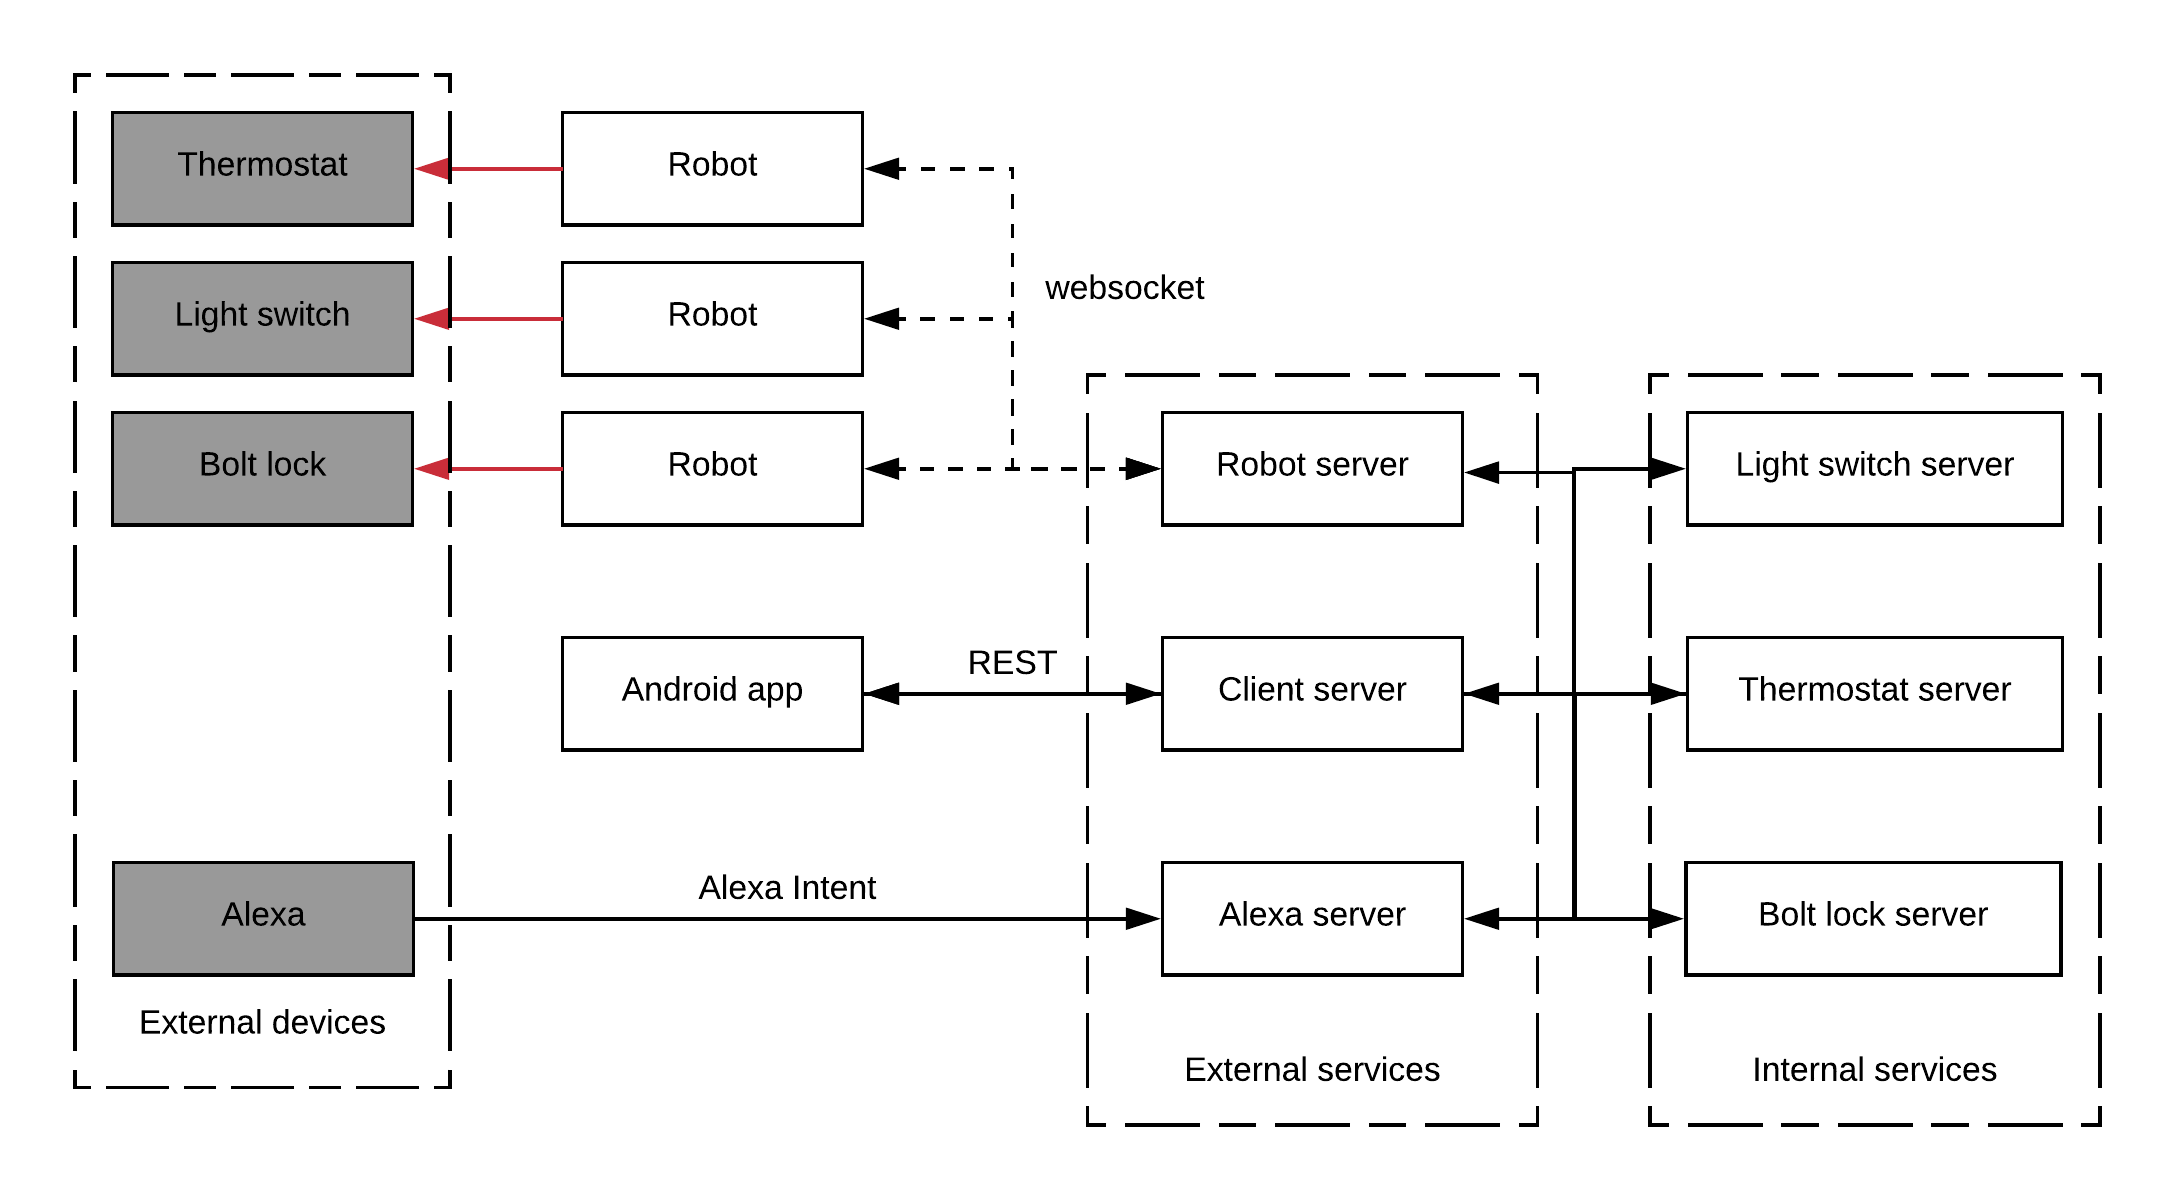
\includegraphics[width=1.0\linewidth]{images/architecture.png}
    \caption{Architecture of our system.}
\end{figure}

\subsection{Robot}

The robot is split into two parts: the controller and the grips. The controller includes an Arduino, an array of sensors, servo and a battery pack. The grips attach to the controller; when the servo turns, the grips manipulate whatever device they are interacting with. The robots themselves attach to the devices with self-adhesive, so that they can easily be removed.

\begin{figure}[H]
    \begin{subfigure}{.5\textwidth}
      \centering
      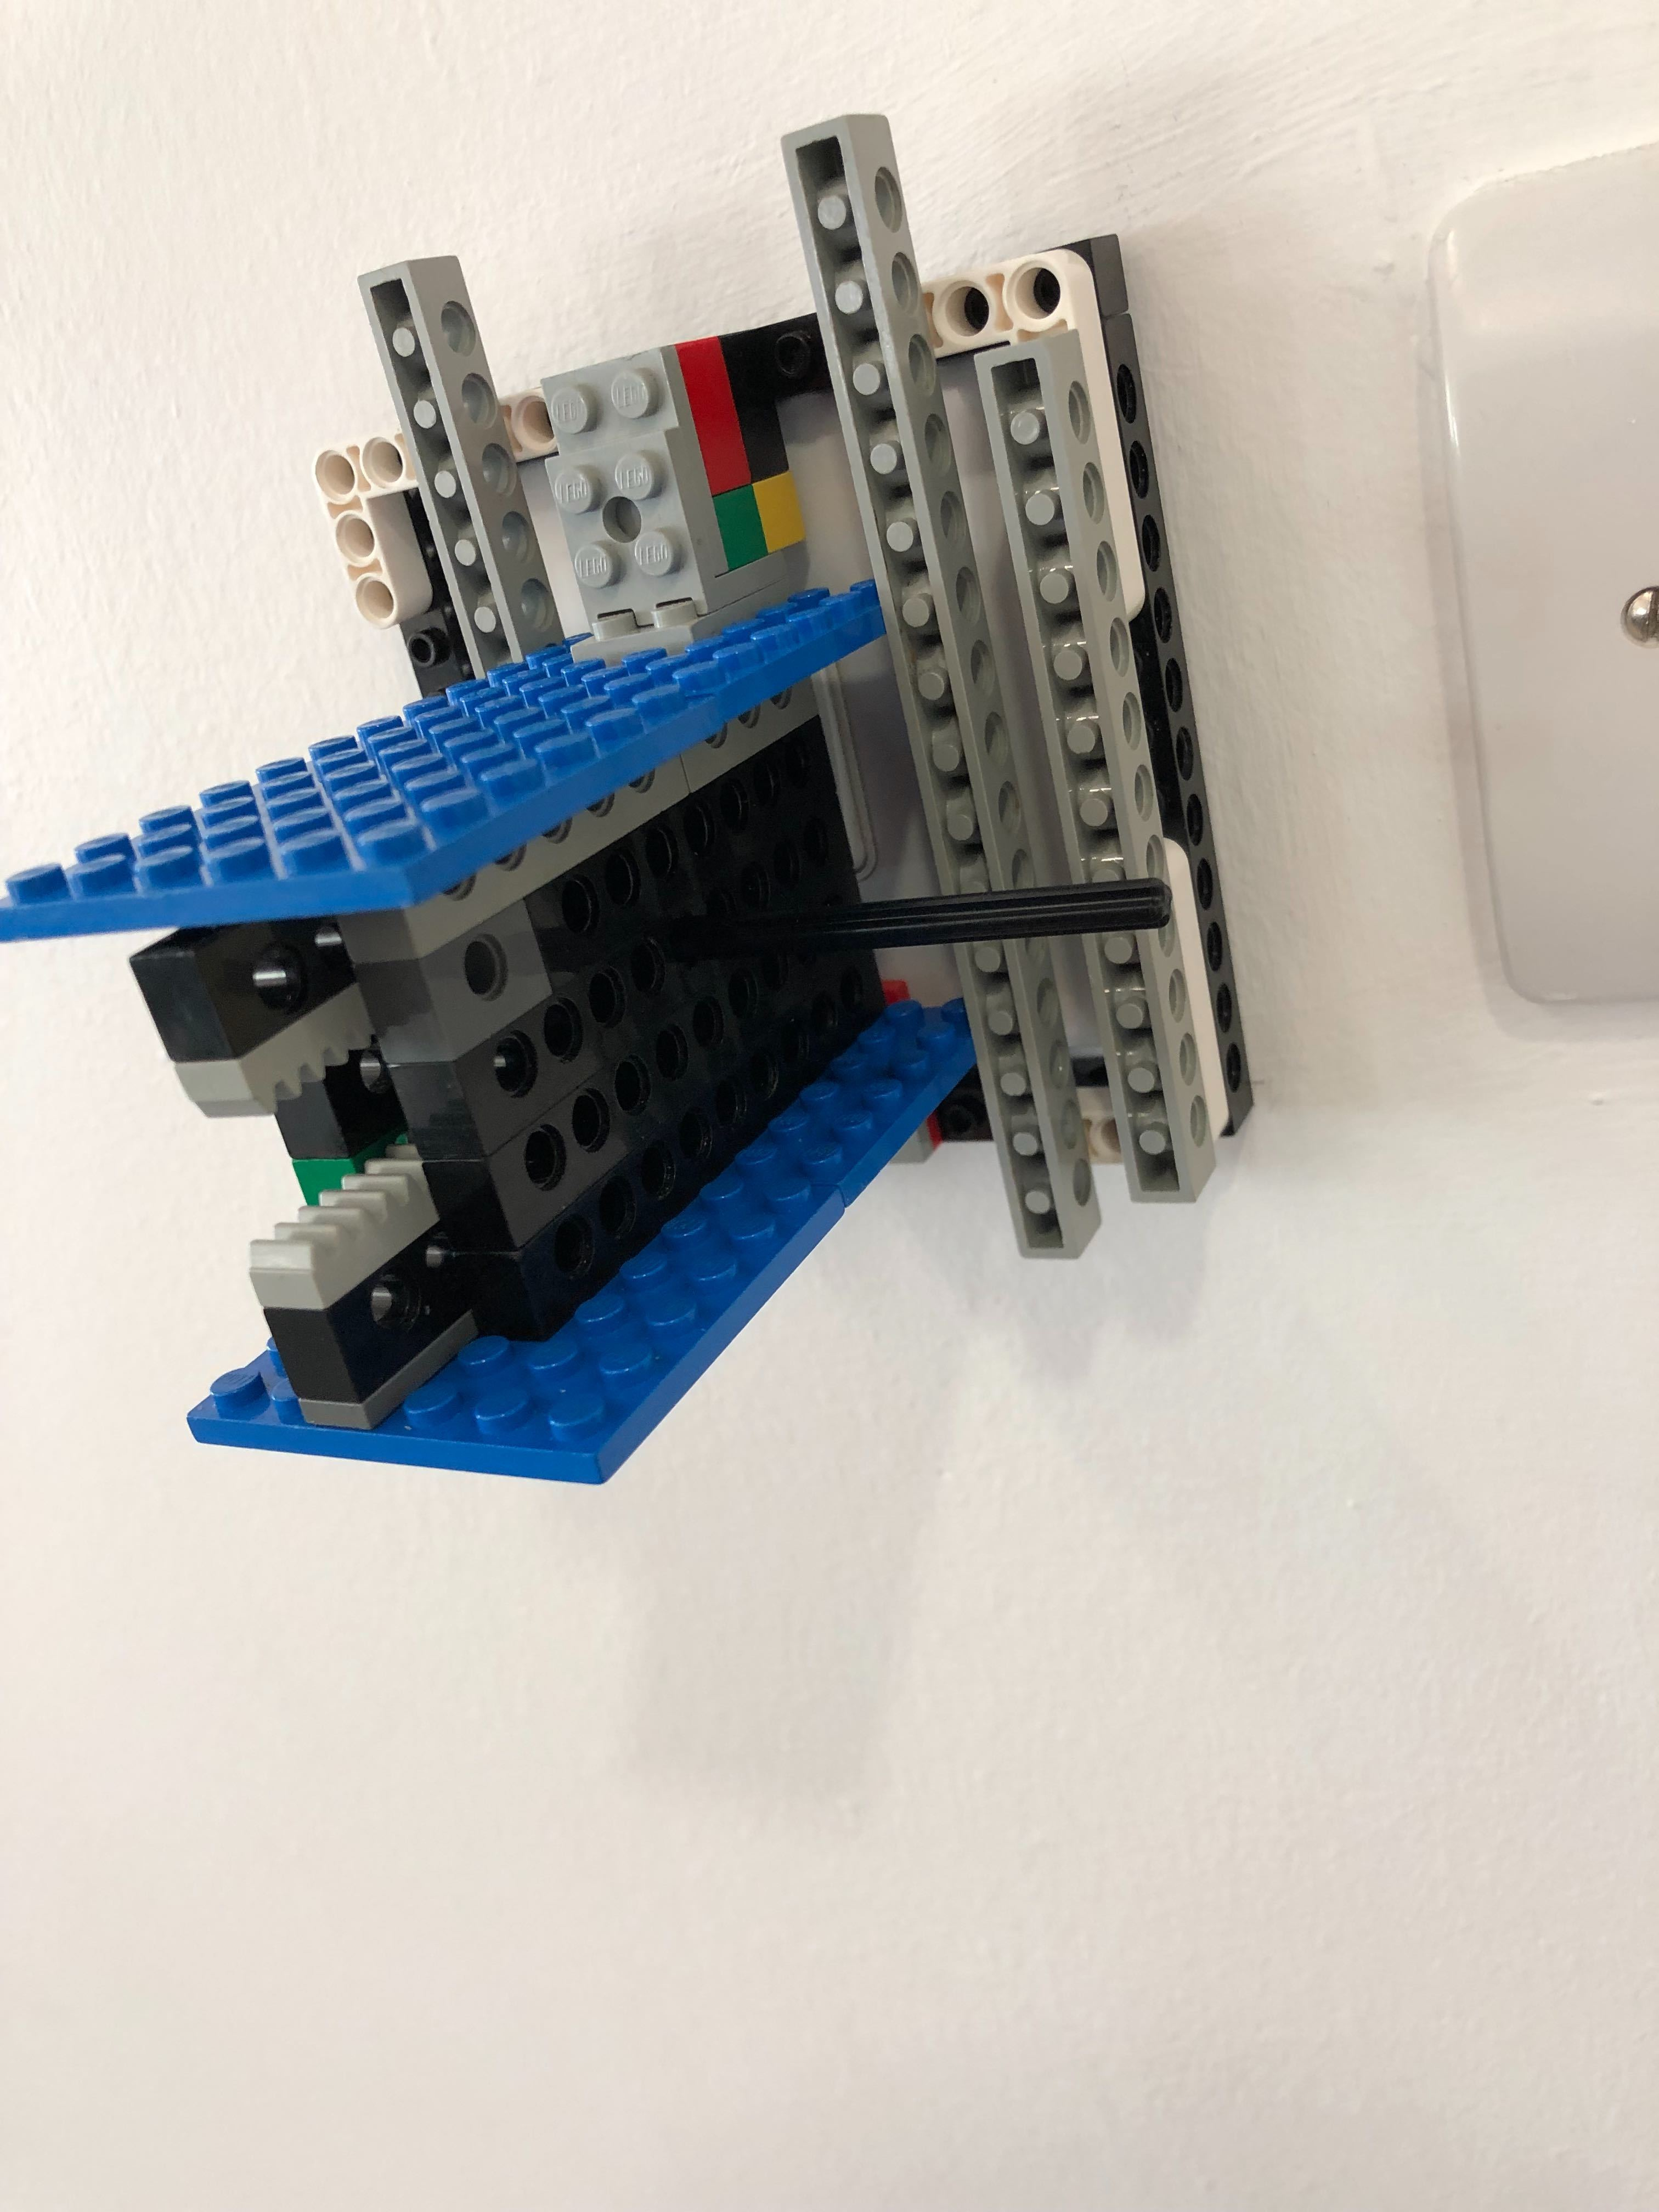
\includegraphics[width=.8\linewidth]{images/light-grip-1.jpg}
    \end{subfigure}
    \begin{subfigure}{.5\textwidth}
      \centering
      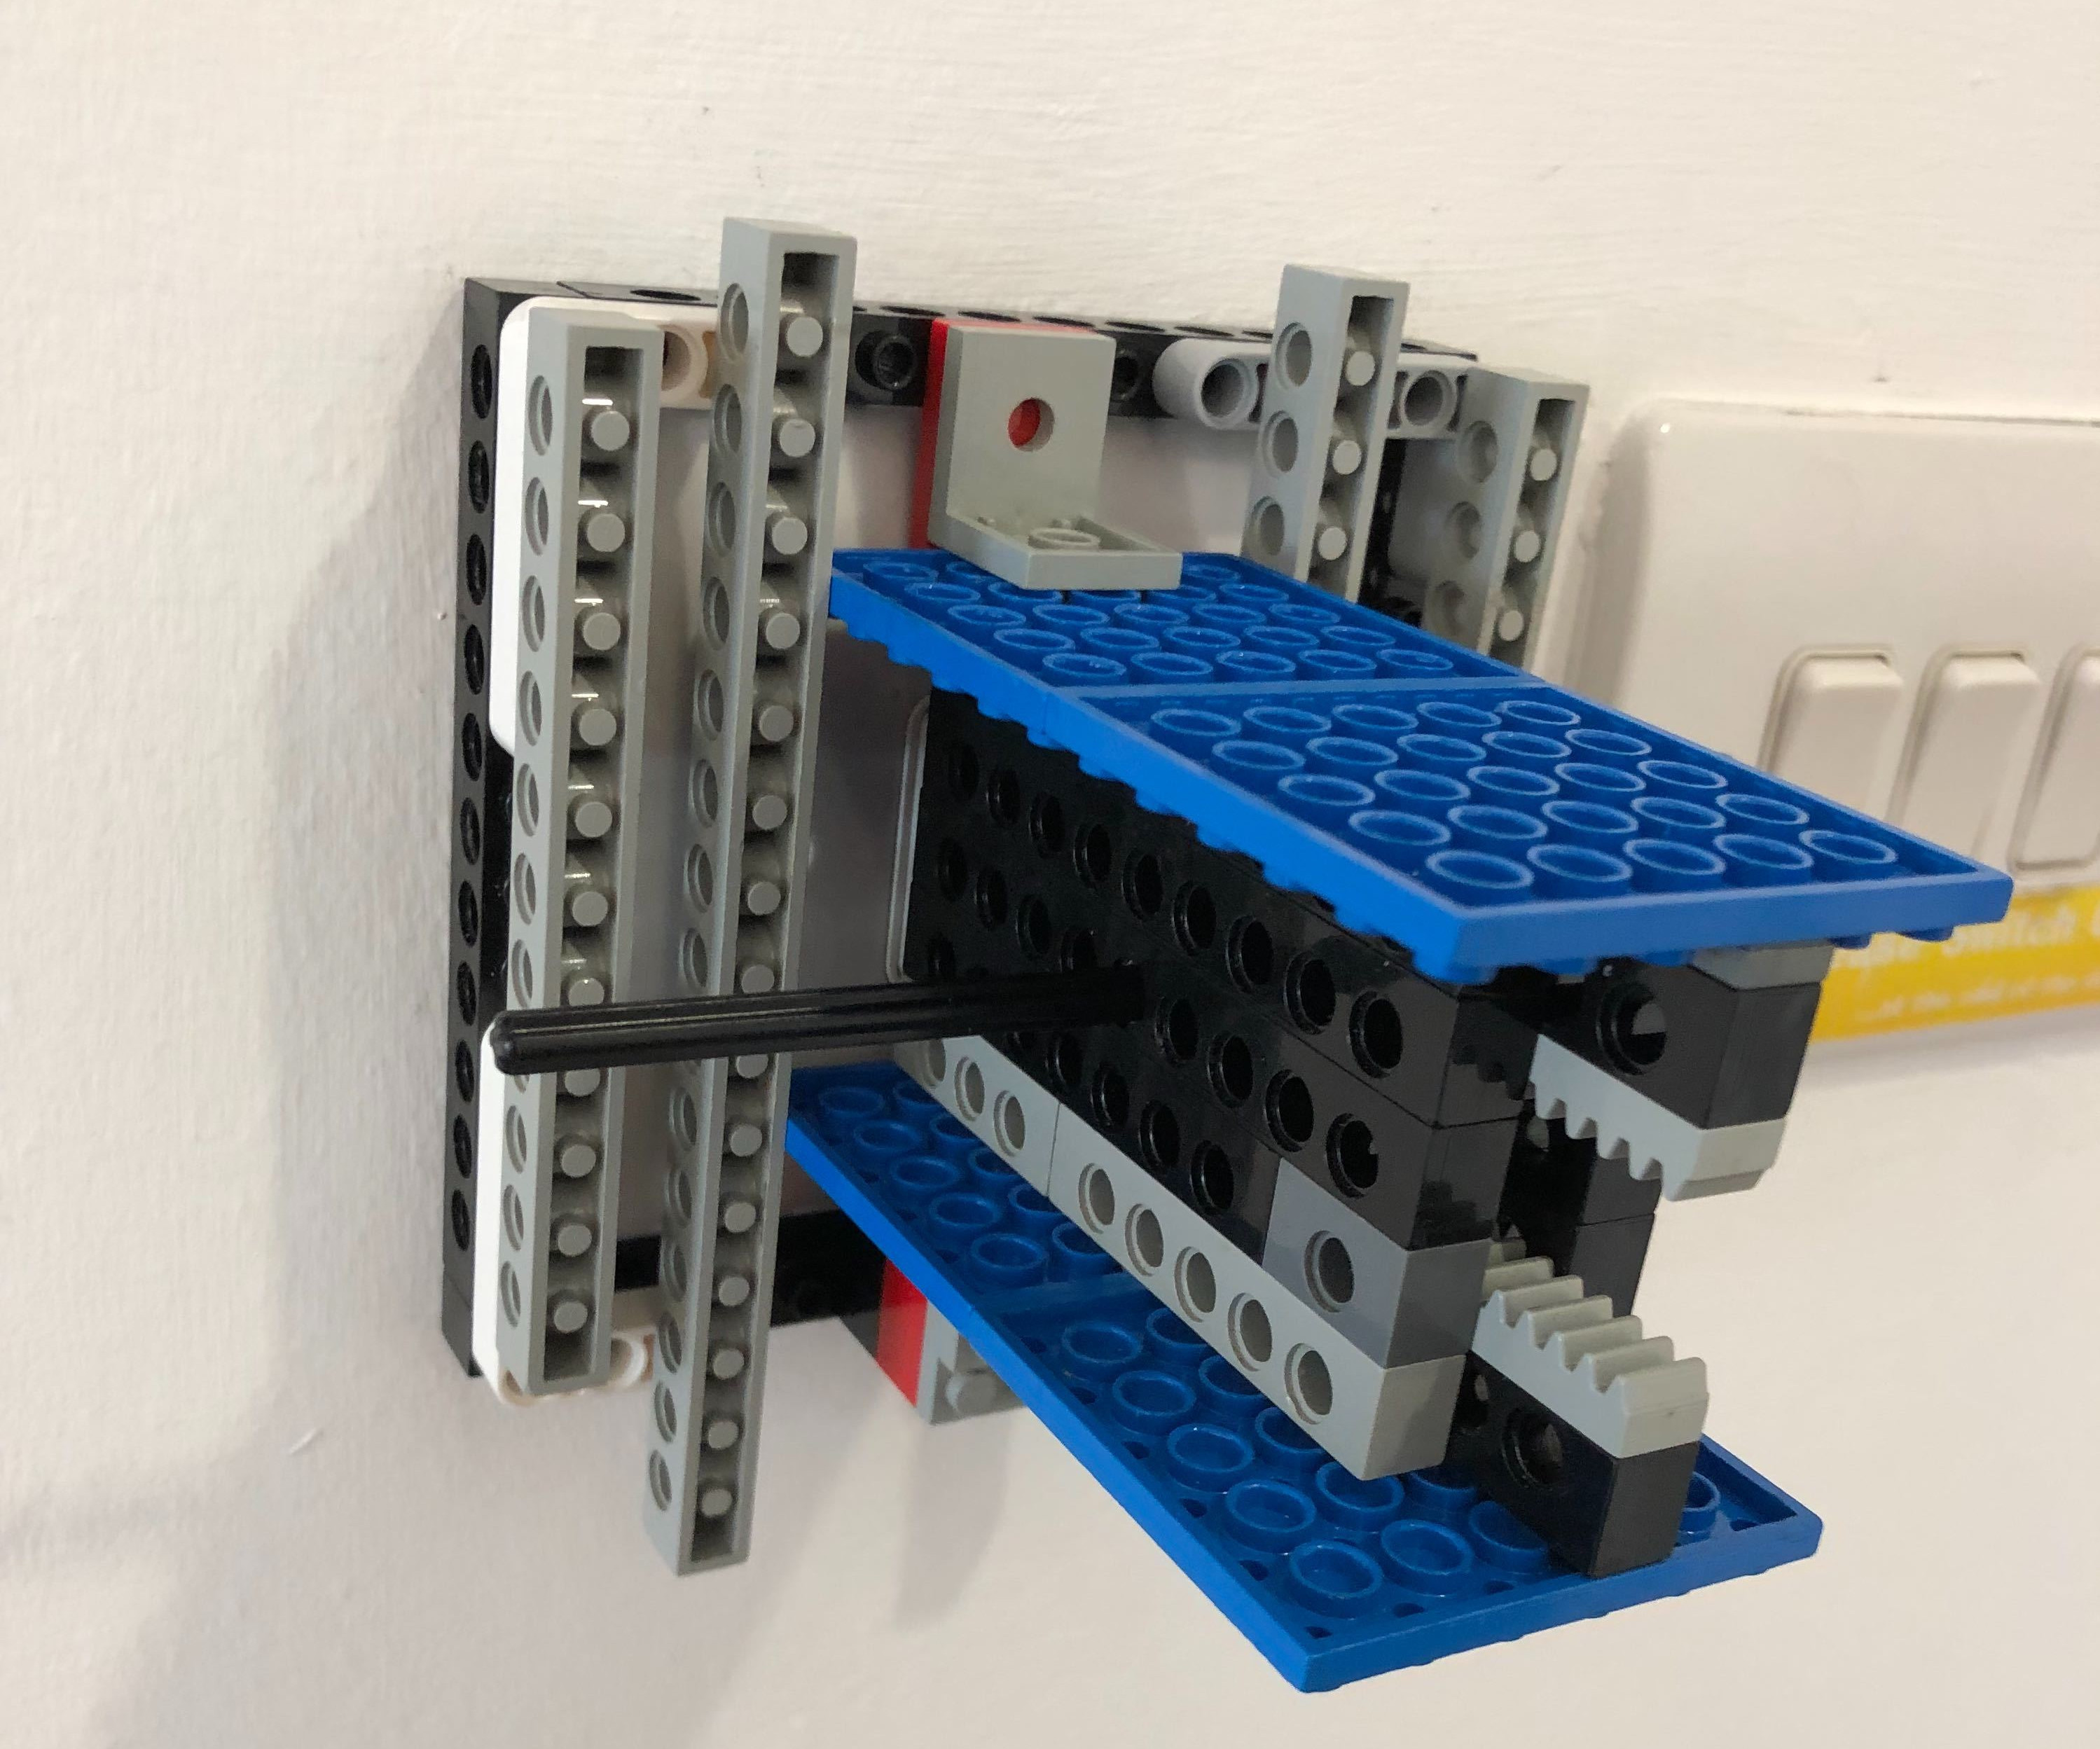
\includegraphics[width=.8\linewidth]{images/light-grip-2.jpg}
    \end{subfigure}
    \caption{First iteration of a light switch grip.}
    \label{fig:fig}
\end{figure}

\subsection{Web server}

The web server is actually a collection of many smaller web servers since we will be following the microservice architecture. The publicly accessible servers are:

\begin{itemize}
    \item The Android app receives data and sends commands via our client API served via the client server. 
    \item Alexa sends Alexa requests to our Alexa server.
    \item The robot is connected via a web socket to the root server.
\end{itemize}

The internal services correspond to each of the use cases. They keep track of the state the device is in, what actions can be performed, and what servo commands need to be sent. This architecture would allow us to point to user made functionality in the future.

\subsection{Android app}

The Android app is the primary user interface into our system. It allows the user to register, calibrate and control their robots.

\begin{figure}[H]
    \begin{subfigure}{.33\textwidth}
      \centering
      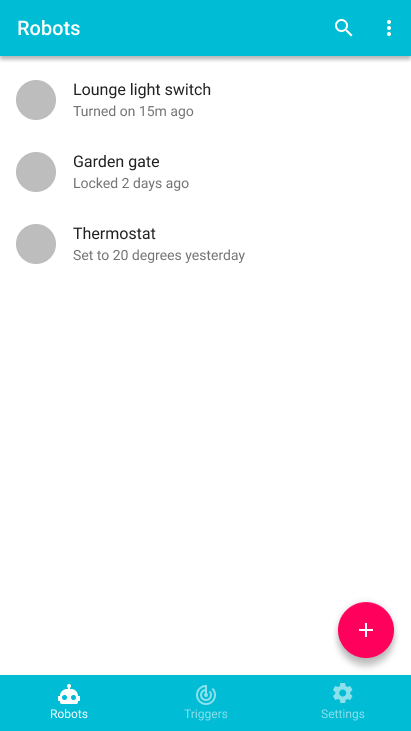
\includegraphics[width=.7\linewidth]{images/app-1.png}
    \end{subfigure}
    \begin{subfigure}{.33\textwidth}
        \centering
        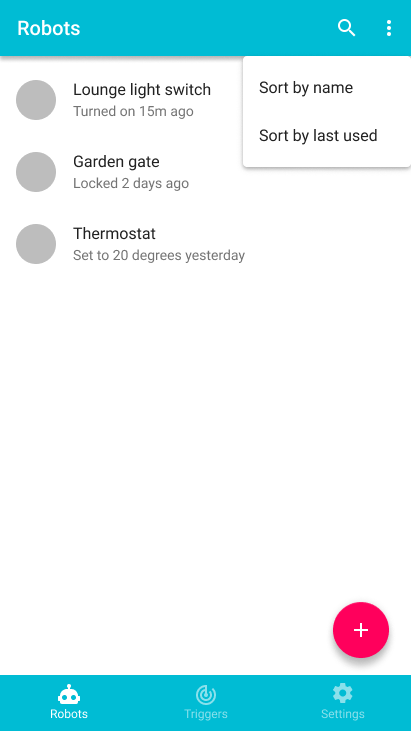
\includegraphics[width=.7\linewidth]{images/app-2.png}
    \end{subfigure}
    \begin{subfigure}{.33\textwidth}
        \centering
        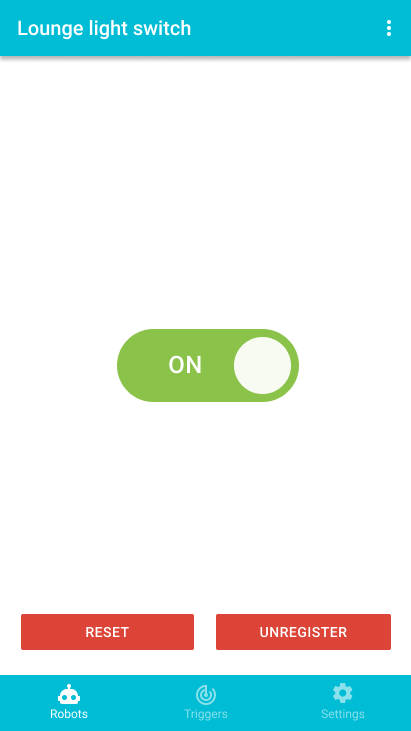
\includegraphics[width=.7\linewidth]{images/app-3.png}
    \end{subfigure}
    \caption{Quick mockup of the Android app.}
    \label{fig:fig}
\end{figure}

\section{Goals}

Our goals are what we want to achieve in each sprint (see organisational structure $\rightarrow$ agile). We aim at having our sprints be approximately two weeks in length, which matches the time between the demos. In each demo we aim to present a few aspects of our system:

\subsection{Demo 1}

\subsubsection{Demo 1.1 - Register and login via the app}

\begin{center}
    \begin{tabularx}{0.8\linewidth}{|c|L|c|}
        \hline
        \textbf{Component} & \textbf{Task} & \textbf{Difficulty} \\
        \hline
        Web server & Register user with email and password & \easy \\
        \hline
        Web server & Authenticate the user and return token & \medium \\
        \hline
        Android & Login/register UI & \easy \\
        \hline
        Android & Send auth token in REST requests & \medium \\
        \hline
    \end{tabularx}
\end{center}

\subsubsection{Demo 1.2 - Switch the light on/off from the Android app}

\begin{center}
    \begin{tabularx}{0.8\linewidth}{|c|L|c|}
        \hline
        \textbf{Component} & \textbf{Task} & \textbf{Difficulty} \\
        \hline
        Web server & Store the state of the switch & \easy \\
        \hline
        Web server & Endpoint for turning light on/off & \easy \\
        \hline
        Web server & Endpoint for retrieving a list of robots & \easy \\
        \hline
        Web server & Establish WebSocket with robot & \easy \\
        \hline
        Web server & Send servo commands on light on/off request & \easy \\
        \hline
        Android & UI to display a list of robots & \easy \\
        \hline
        Android & Light switch toggle UI & \medium \\
        \hline
        Android & Send light on/off request & \medium \\
        \hline
        Robot & Establish websocket with server & \easy \\
        \hline
        Robot & Receive servo commands & \medium \\
        \hline
        Robot & Construct the LEGO switch gripper & \medium \\
        \hline
        Robot & Connect the servo to Arduino & \easy \\
        \hline
        Robot & Create temporary client on DICE to forward servo commands (since the Arduino we have doesn’t have a Wifi chip) & \medium \\
        \hline
    \end{tabularx}
\end{center}

\subsection{Demo 2}

\subsubsection{Demo 2.1 - Walkthrough the robot registration process}

\begin{center}
    \begin{tabularx}{0.8\linewidth}{|c|L|c|}
        \hline
        \textbf{Component} & \textbf{Task} & \textbf{Difficulty} \\
        \hline
        Web server & Endpoint to register a robot to the users account & \easy \\
        \hline
        Web server & Only return the list of robots registered to the user's account & \easy \\
        \hline
        Android & UI for registering a new robot & \hard \\
        \hline
        Robot & Assign each robot a hard-coded ID & \easy \\
        \hline
    \end{tabularx}
\end{center}

\subsubsection{Demo 2.2 - Demonstrate robot calibration steps on the app}

\begin{center}
    \begin{tabularx}{0.8\linewidth}{|c|L|c|}
        \hline
        \textbf{Component} & \textbf{Task} & \textbf{Difficulty} \\
        \hline
        Web server & Endpoint to send calibration parameters including a range, min and max values & \easy \\
        \hline
        Web server & Endpoint to receive calibration parameters & \easy \\
        \hline
        Android & Dynamically build UI for calibrating the robot & \hard \\
        \hline
        Android & Send calibration parameters back to the server & \medium \\
        \hline
    \end{tabularx}
\end{center}

\subsubsection{Demo 2.3 - Adjust temperature via the Android app}

\begin{center}
    \begin{tabularx}{0.8\linewidth}{|c|L|c|}
        \hline
        \textbf{Component} & \textbf{Task} & \textbf{Difficulty} \\
        \hline
        Web server & Store current temperature settings & \easy \\
        \hline
        Web server & Endpoint to get the current temperature & \easy \\
        \hline
        Web server & Endpoint to update the current temperature & \easy \\
        \hline
        Android & UI to choose the desired temperature & \easy \\
        \hline
        Android & Send the desired temperature to the server & \medium \\
        \hline
        Robot & Construct the LEGO dial grip & \hard \\
        \hline
    \end{tabularx}
\end{center}

\subsection{Demo 3}

\subsubsection{Demo 3.1 - Physical demonstration of 3D printed version}

\begin{center}
    \begin{tabularx}{0.8\linewidth}{|c|L|c|}
        \hline
        \textbf{Component} & \textbf{Task} & \textbf{Difficulty} \\
        \hline
        Robot & 3D print case for controller & \hard \\
        \hline
        Robot & 3D print light switch grip & \hard \\
        \hline
    \end{tabularx}
\end{center}

\subsubsection{Demo 3.2 - Asking Alexa to turn a light switch on}

\begin{center}
    \begin{tabularx}{0.8\linewidth}{|c|L|c|}
        \hline
        \textbf{Component} & \textbf{Task} & \textbf{Difficulty} \\
        \hline
        Web server & Create Alexa skills schema & \easy \\
        \hline
        Web server & Add Alexa endpoints for receiving Alexa requests & \hard \\
        \hline
    \end{tabularx}
\end{center}

\subsubsection{Demo 3.3 - Present unlocking and locking a bolt lock via the app}

\begin{center}
    \begin{tabularx}{0.8\linewidth}{|c|L|c|}
        \hline
        \textbf{Component} & \textbf{Task} & \textbf{Difficulty} \\
        \hline
        Web server & Endpoint for unlocking/locking bolt lock & \easy \\
        \hline
        Android & UI for unlocking/locking bolt lock & \easy \\
        \hline
        Android & Send request to lock/unlock bolt lock & \medium \\
        \hline
        Robot & Build grip to manipulate bolt lock & \hard \\
        \hline
    \end{tabularx}
\end{center}

\subsection{Demo 4 (Final Demo)}

\subsubsection{Demo 4.1 - Demonstrate push notification on low battery}

\begin{center}
    \begin{tabularx}{0.8\linewidth}{|c|L|c|}
        \hline
        \textbf{Component} & \textbf{Task} & \textbf{Difficulty} \\
        \hline
        Web server & Create a push notification server & \easy \\
        \hline
        Web server & Receive battery status from the robot and send a push notification when robots battery is low & \easy \\
        \hline
        Android & Register for push notifications with the Android OS & \easy \\
        \hline
        Robot & Send battery status over WebSocket & \easy \\
        \hline
    \end{tabularx}
\end{center}

\subsubsection{Demo 4.2 - Demonstrate turning a light switch on when it’s dark}

\begin{center}
    \begin{tabularx}{0.8\linewidth}{|c|L|c|}
        \hline
        \textbf{Component} & \textbf{Task} & \textbf{Difficulty} \\
        \hline
        Web server & Store sensor data sent from the robots & \medium \\
        \hline
        Web server & Endpoint for requesting history of the sensor data & \medium \\
        \hline
        Web server & Create endpoints for adding/deleting/updating triggers & \medium \\
        \hline
        Web server & When a triggers condition is met send the servo command & \easy \\
        \hline
        Android & UI for configuring a trigger & \easy \\
        \hline
    \end{tabularx}
\end{center}

\subsection{Extensions}

If there is time remaining at the end of the project, there are a number of extensions we could add.

\begin{itemize}
    \item \textbf{Fall detection:} Using an accelerometer, we could detect if the device falls off the wall and send the user a notification.
    \item \textbf{iOS app:} An iOS app would allow us to integrate with Siri and the Apple Home app. It would also expand our market.
    \item \textbf{Web app:} Allow for remote control from anywhere without installing an app.
    \item \textbf{Android app (extensions):} Google Home \& Bixbe integration would bring voice control to more devices.
    \item \textbf{If this then that:} IFTTT is a popular tool for making smart home devices work together. Integrating with IFTTT will provide a more cohesive smart home experience.
    \item \textbf{Machine learning:} Using sensor data we could automatically discover rules such as:
        \begin{itemize}
            \item Turn the heating on if it's below 16 degrees celsius
            \item Turn the lights off at 11 pm
            \item Etc
        \end{itemize}
    \item \textbf{Developer API and the marketplace:} We could provide an API so users can use the hardware in new and creative ways. The marketplace would allow developers to list their extensions and users to discover new applications for our device.
    \item \textbf{Product website:} It would be nice to have a product website to enhance our stand at the trade fair. It would include:
        \begin{itemize}
            \item Developer API documentation
            \item Shopping cart and product selection functionality
            \item Product showcase
        \end{itemize}
\end{itemize}

\section{Time planning}

\begin{figure}
    \centering
    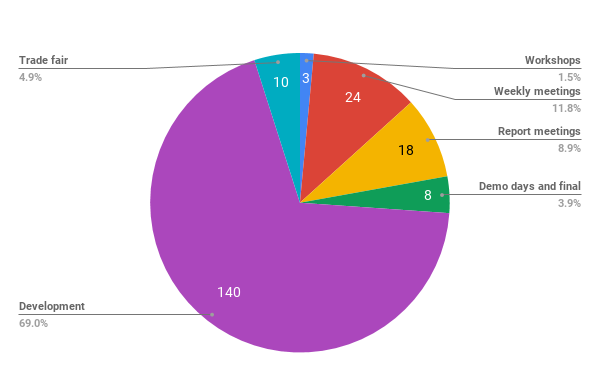
\includegraphics[width=0.8\linewidth]{images/time.png}
    \caption{Breakdown of how many hours each of our team members will spend on various aspects of the project.}
\end{figure}

\subsection{Time breakdown}

\subsubsection{Workshops}

Not everyone is sure what workshops they want to attend, so we are allocating 3 workshops (3 hours) per person.

\subsubsection{Weekly meetings}

Weekly meetings will occur on a Monday from 15:00 to 17:00. The first half of each meeting will also include our mentor.

\subsubsection{Report meetings}

Besides the weekly meetings, we will have three 2 hour meetings for each report.

\subsubsection{Demo days and final presentations}

We will allocate 2 hours per demo, this including time to prepare for the demo and time to reflect on the feedback we get afterwards.

\subsubsection{Trade fair}

The trade fair is from 9:00 till 17:30, but we will also be allocating another 2 hours to ensure our robot and display is ready.

\subsubsection{Development}

The rest of our time will be working on our assigned components (see organisational structure $\rightarrow$ components). This work includes building, programming, testing, bug fixing and code reviews. There are 28 easy tasks, 13 medium tasks and 7 hard tasks. If we allocate 10 hours for easy tasks, 20 hours for medium tasks and 30 hours for hard tasks we get 750 hours in total out of the 980 working hours we have available. This leaves us with plenty of time in case we have underestimated the complexity of some goals.

\subsection{Skills}

\subsubsection{Web services}

The web server is the largest most complex part of our system, however both Ben and Gwion have produced similar sized web services in the past. Ben recently worked on a prototype event system for the UoE during an internship. Gwion has developed several web services for the UoE during an internship and as part-time work.

\subsubsection{Android}

A large majority of the team have had experience working on mobile apps through ILP, and a couple of team members have experience outside of university: Ben developed a fully featured mobile GitHub client, and Luke has some experience with Swift if we decide to port the app to iOS. We are therefore confident that we already have the skills necessary to complete the easier tasks such as \textit{UI to display a list of robots} (demo 1.2). Goals such as \textit{Register for push notifications with the Android OS} (demo 4.1) will require some research, however we are familiar with the Android documentation so we know where to look.

\subsubsection{Hardware}

Luke has worked on FTC robots for four years; while it wasn’t LEGO he is confident his skills will be transferable. Spencer and Sameer have experience with electronics as part of their degrees.

\subsubsection{3D printing}

A few members of the team have done some 3D modelling before. Wang has 3D printed some simple cases over the break.

\subsection{Gantt Chart}

% TODO: insert gantt chart

\section{Risks}

\begin{center}
    \begin{tabularx}{1.0\linewidth}{|L|L|L|L|L|}
        \hline
        \textbf{Risk} & \textbf{Impact} & \textbf{Likelihood} & \textbf{Actions to take to minimize the risk} & \textbf{Contingency plan} \\
        \hline
        The servos might not be powerful enough to interact with the switches and thermostats. & Severe - We are unable to operate some or all devices such as switches or thermostats. & Low - Our use cases don't require a lot of force, so fairly week servos should still work. & Prototype the first iteration of grips as early as possible to leave more time for alternative approaches. & Order more powerful servos, possibly delaying the first demonstration of light switching until demo 2. \\
        \hline
        It might be difficult to grip the switches and dials. & Severe - We are unable to manipulate the switches and dials. & Low - Our initial tests suggest this shouldn't be a problem. & Prototype the first iteration of grips as early as possible to leave more time for alternative approaches. & Order/construct more powerful gripper materials, possibly delaying the first demonstration of light switching until demo 2. \\
        \hline
        It may end up being too costly for us to develop several adapters. & Moderate - We will not be able to demonstrate the system’s true potential in the demos. & Low - The parts list we have made (see below) seems sensible. & Use the materials already available to the furthest extent possible, even if it means some inconsistency in the platform. & We will scale back the number of devices we are showcasing at once. We can reuse the controllers themselves but switch out the grips during the demo, thus we can still showcase the versatility of our product. \\
        \hline
        There is a risk that we don’t have the skills and/or budget to design and 3D-print parts to replace the LEGO construction. & Minor - The adapters will be larger, clunkier, and uglier, making the prototypes less impressive. & High - it is a complex task and most of the team is inexperienced in this area. & Communicate with Gary to discuss what costs are involved; allow plenty of time for the design process. & Stick with the LEGO. \\
        \hline
        The devices draw a lot of power and need to be recharged very frequently. & Moderate - The convenience of remote control would be overshadowed by the time spent charging the devices, making the product unattractive. & Unknown - Without previous experience it is hard to judge how likely it is that this problem will arise. & By using Arduinos and offloading most of the logic onto the server we hope to reduce power draw. & We will pivot to use cases where we can assume the user has a power outlet nearby such as the thermostat. \\
        \hline
        A lack of skills may mean we cannot complete the project with Arduinos, which is arguably the most complex platform due to its low-level nature. & Moderate - We may only be able to build a few controllers and they would be many times larger than we had envisioned due to the size of the alternative platforms. & Low - There is not a lot of complexity in the robot code, so we should be able to work through the issues that arise. & Start building the adapters early, communicate clearly with the rest of the team on Slack and in the weekly meetings if there are issues. & We will move to the EV3 platform. \\
        \hline
        A lack of skill may mean we cannot complete the web server. & Moderate - We will have to offload large parts of the logic to the app (making it harder to port to other systems such as iOS in the future) and the robots (increasing power draw). & Low - Gwion and Ben both have experience developing similar systems. & We have identified that Gwion and Ben are experienced in this area and have allocated the related tasks accordingly. & We will either allocate more people to work on the web server, or offload some of the logic to the robot and/or Android app. \\
        \hline
        A lack of skill may mean we cannot complete the Android app. & Severe - The user will not be able to control or set up the robots from their phone. & Low - thanks to ILP most of the team have relevant experience. & We have allocated three members, all of whom took ILP, to work full or part-time on this component. & We will switch to building a web app. A web app has a number of advantages (namely that there is no installation) and disadvantages (less convenient for the user). \\
        \hline
        We will be using the same self-adhesive as stick-on hooks to attach our robot to the users' device. If the robot is too heavy, the self-adhesive may not be able to hold the weight. & Severe - The robots will not stay attached to the walls, making them unusable for most use cases. & Low - the components we are planning to use are quite light, and self-adhesive strips can take quite a bit of weight. & Trial this early in the development process and make sure to thoroughly test it for all types of grippers. & We will increase the surface area of the robot so we can fit larger self-adhesive pads, or look into using suction cups instead if appropriate. \\
        \hline
    \end{tabularx}
\end{center}

\section{Organisational structure}

\subsection{Team leaders}

Both Luke Drennan and Ben Sheffield will function as team leaders. Luke has 4 years of robotics experience and will focus on the robotic component of the project. Ben has experience with managing large git repositories and also has a lot of free time. Ben is also the designated group contact.

\subsection{Treasurer}

Theo Olausson will be the treasurer for the project. A Google Sheet with communal access has been set up so that any member of the group can see how much of the budget remains and suggest purchases, however, these suggestions must be accepted by Theo and the team leaders before going through. This way the group will stay in control of the budget at all times.

\begin{center}
    \begin{tabularx}{\linewidth}{|l|c|c|L|}
        \hline
        \textbf{Item} & \textbf{Quantity} & \textbf{Total} & \textbf{Notes} \\
        \hline
        AWS & 1 & £20 & We should only need the free tier for the web server. However we have allocated £20 in case we have underestimated our compute needs. \\
        \hline
        halspals.co.uk domain & 1 & £6 &  \\
        \hline
        ESP8266 & 3 & £20 & Incredibly small Arduino-compatible board with WiFi chip. Has a large community with lots of resources available. \\
        \hline
        Servos & 3 & £15 & Rough estimate as we are not sure exactly what servos we will need; will need to experiment with the LEGO servos first. \\
        \hline
        Light sensor & 3 & £5 &  \\
        \hline
        3D printing &  & £50 & We will need to go through a couple of iterations before we get the right fit, so we are allocating a lot of our budget just in case. \\
        \hline
        Self adhesive pad & & £10 & For attaching robots to devices.\\
        \hline
        Light switch & 1 & £5 & For demonstration purposes.\\
        \hline
        Basic thermostat & 1 & £10 & For demonstration purposes.\\
        \hline
        Bolt lock & 1 & £10 & For demonstration purposes.\\
        \hline
        Echo dot & 1 & £30 & If possible we would like to get a cheaper refurbished/used one. \\
        \hline
    \end{tabularx}    
\end{center}

The total arrives at £181. We don't expect to spend this much; we have been generous with prices in this table in case the parts turn out to be more expensive than the ones we have found on Amazon.

\subsection{Components}

Our system is split into 3 main components: web server, Android app, and the robots. The following is a breakdown of who will be focusing on what, though we encourage all team members to make themselves useful across all the components:

\begin{itemize}
    \item \textbf{Web server:} Ben, Gwion, Wang (Alexa integration)
    \item \textbf{Android app: } Theo, Ben (UI Design), Han
    \item \textbf{Robot: } Luke, Spencer, Wang, Han, Sameer
\end{itemize}

\subsection{Git \& GitHub}

We have decided on using Git for version control, with GitHub as our host. GitHub has a number of features such as code review and triage tools nicely integrated. Issues and pull requests can be assigned a deadline so we can easily view what needs to be done before the next demo across the 3 components, and how we are progressing. We decided against using Trello since there is nothing Trello offers that we want or GitHub projects don’t already offer.

The repository will be a monorepo (all the components exist in the same repository). It makes it much easier to do multi-component refactoring such as changing a REST endpoint. Regarding workflow, we are using a simplified version of git-flow, since we don’t need the overhead of versioning (we are only creating a prototype).

When creating a feature, we will branch from the relevant component branch and create a pull request back into the component branch. Before the pull request is accepted Travis (our chosen Continuous Integration system) will run the test suites to check for problems, and another team member will perform a code review. It will help to catch bugs and makes sure everyone's code is readable.

At least three days before a demo we will have a group meeting where we will merge the component branches into master. As a group, we can then fix any integration issues between the 3 components on the spot.

\subsection{Agile}

For this project, we have decided that we will be loosely following Agile practices. Considering that we will have the team working on different components, we need to prevent one area being held back waiting for another. Thus communication practices of Agile such as the daily standup are especially helpful; team members must say what they have done, what they will do, and if they need help or are being hindered. 

Our sprints will be approximately two weeks in length, so that they may match the time between demos. Our progress will be tracked at the beginning/end of each sprint, allowing us to review the efficiency of the team and better set our goals for the next sprint and demo.

\subsection{Meetings}

Meetings are scheduled on google calendar and slack, so everyone knows what's happening and when. We will also be keeping a log of what was discussed at meetings. Firstly, if someone could not make it to the meeting, they can check the meeting log to see what was discussed. Secondly, it will help later when writing our reports.

\end{document}
